\chapter{Post-Quanten-Kryptografie Signatur Algorithmen}
\label{section-Post-Quanten-Kryptografie-algorithmen}
Durch die mögliche Bedrohung von Quantencomputern in der Zukunft, werden neue Kryptographische Verfahren standartisiert.
Das NIST hat dabei fünf Sicherheitsstufen definiert als Referenz welches Niveau für die Algorithmen zu erbringen ist.
Die Sicherheitsstufen und deren Referenz sind in Abbildung-\ref{fig:NIST-Sicherheitslevel} zu sehen\cite{soniHardwareArchitecturesPostQuantum2021}.

\begin{table}[htbp]
    \centering
    \begin{tabular}{|c|c|c|>{\centering\arraybackslash}p{3.5cm}|}
        \hline
        Sicherheits Level & Vergleich & Angriffsverfahren & Ressistenz gegen Quantencomputer\\
        \hline
        1 & $\ge$ AES128 & vollständige Schlüsselsuche & schwach\\
        \hline
        2 & $\ge$ SHA256 & Kollisionsangriff & stark\\
        \hline
        3 & $\ge$ AES192 & vollständige Schlüsselsuche & stärker als Level 1 oder 2\\
        \hline
        4 & $\ge$ SHA384 & Kollisionsangriff & sehr stark\\
        \hline
        5 & $\ge$ AES256 & vollständige Schlüsselsuche & stärkste Ressistenz\\
        \hline
    \end{tabular}
    \caption{NIST Sicherheitslevel für PQC-Verfahren}
    \label{fig:NIST-Sicherheitslevel}
\end{table}

\section{Der Umstieg von derzeitigen Digitalen Signaturen zu PQC}
Die heutigen Digitalen Signaturen ((EC)DSA, (EC)ElGamal) basieren auf dem diskreten Logarithmus Problem oder bei RSA auf der schwierigkeit des faktorisierens großer Semi-Primzahlen in dessen Primfaktoren.
RSA hat den Vorteil, dass die verschlüsselung und die Signatur sich nicht stark von einander unterscheiden.\cite{paarKryptografieVerstaendlichLehrbuch2016}

Die Verfahren aus dem NIST-Auswahlprozess haben längere Signaturen und nicht so einfach wie RSA.
Der Signatur- und Verschlüsselungsalgorithmus unterscheiden sich stärker voneinander. Für DNSSEC sind nur die Signaturen interessant.

\section{NIST Auswahlprozess für Digitale Signaturen}
Zur Zeit dieser Arbeit befindet sich der NIST Auswahlprozess in der 4-ten Runde, nach dem Stand vom 11.März.2025.
Als digitalen signatur Standart zugelassen sind momentan CRYSTALS-Dilithium (ML-DSA), FALCON (FN-DSA) und SPHINCS$^+$ (SLH-DSA) \cite{alagicStatusReportFourth2025}.
Zusätzliche Kandidaten für Digitale Signatur Schemas, die noch standartisiert werden sollen, sind noch in der evalution.
Anfang der dritten Runde waren noch  FAEST, HAWK, MAYO, MQOM, QR-UOV, SDitH, SNOVA, SQIsign, und UOV vorhanden \cite{moodyStatusReportSecond2026}.

\subsection{Crystals-Dilithium}
Das von der NIST favorisierte Verfahren, es wurde unter anderem von Deutschen Kryptographen entwickelt und basiert auf der schwierigkeit den nächsten Gitterpunkt zu einem Punkt in einem Hochdimensionalem Gitter zu finden.
Es wird ein Gleichungssystem aufgestellt für das eine Lösung mit kleinen Zahlen gefunden werden muss.
Es basiert auf dem Short Integer Solution (SIS) Problem.
Das Gleichungssystem, welches auch der öffentliche Schlüssel ist, enthält zudem kleine Fehler.
Der private Schlüssel ist die Lösung dieses Gleichungssystems.
Um aus der Einwegfunktion (aufstellen eines fehlerhaftes Gleichungssystems) ein valides Kryptosystem zu bauen, wird die sog. Fiat-Shamir Funktion angewandt.
Wenn die Einwegfunktion sich auch mit Quantencomputern nicht effizient lösen lässt, ist das Verfahren durch die Fiat-Shamir-Transformation Quanten sicher.\cite{schmehFiatShamirTransformation2026,schmehGitterbasierteAlgorithmen2026}

\begin{figure}[htbp]
    \centering
    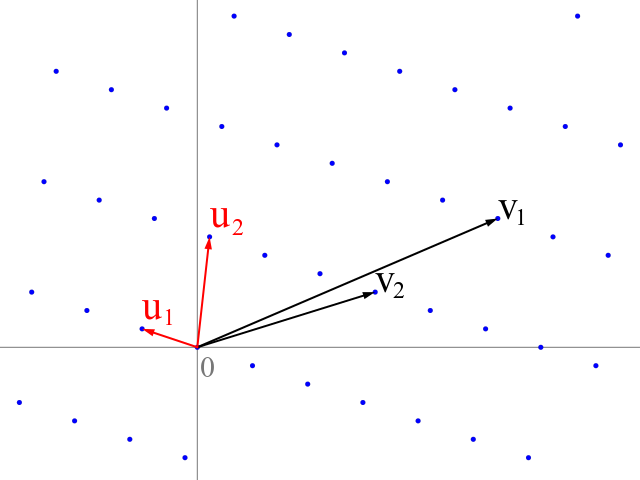
\includegraphics[width=0.5\textwidth]{bilder/lattice-reduction-3867677526.png}
    \caption{2-dimensionales Gitter mit einem Punkt und dem nächstgelegenen Gitterpunkt \cite{barakIntensiveIntroductionCryptography}.}\hfill
    \label{fig:gitter-sis}
\end{figure}

Abbildung \ref{fig:gitter-sis} zeigt das SIS-Problem in einem zweidimensionalen Gitter.
Von dem Punkt $V_1$ aus soll der nächstgelegene Gitterpunkt $V_2$ gefunden werden, die Basisvektoren $(u_1,u_2)$ stellen eine schlechte Basis bereit.
Es muss ein höherdimensionales Gitter und eine schlechte Basis verwendet werden, damit das Problem schwer genug ist\cite{schmehGitterbasierteAlgorithmen2026}.

\subsection{FALCON}
\textbf{Fa}st-Fourier \textbf{L}attice-based \textbf{Co}mpact Signatures over \textbf{N}TRU, kurz \textbf{FALCON}.
Das einzige dieser Kryptosystem, welches mit Gleitkommzahlen rechnet.
Es basiert auch auf dem Short Integer Solution (SIS) Problem über NTRU Gittern \cite{Falcon}.
FALCON gilt aufgrund von Gleitkommazahlen, rekursiven Funktionen und mehreren diskreten Gaussverteilungen als schwerig zu implementieren.
FALCON hat den Vorteil, dass es kleine Signaturen und öffentliche Schlüssel hat und das es schneller im verifizieren ist.
Unter anderem nutzt es die Fast-Fourier-Transformation mit einer Superlinearen Laufzeitkomplexität von $O(n \log n)$ anstelle der Fourier-Transformation mit einer quadratischen Laufzeitkomplexität $O(n^2)$.\cite{nguyenFastFalconSignature2023,soniFALCON2021}
Crystals-Dilithium und FALCON nutzen zur Verifikation \enquote{Fiat-Shamir with aborts}, welches ein challenge-response Verfahren ist\cite{LatticeSignaturesFiatShamir}.

\subsection{SPHINCS$^+$}
Ein konservatives Verfahren, welches auf der Sicherheit von Hashfunktionen aufbaut.
Da Hashfunktionen gut erforscht sind und nicht anfällig sind durch Shor's Algorithmus und Grover's Algorithmus die Sicherheit nur bedingt beeinträchtigt, gelten sie als ziemlich sichere Alternative.
SPHINCS$^+$ ist eine modifizierte Version von SPHINCS und ein sogenanntes \enquote{zustandloses Signaturverfahren}.
Es unterstützt die Hashfunktionen, SHAKE und SHA, zudem in unterschiedlichen Längen und als short oder fast.
Intern funktioniert dieses Verfahren auch mit Merkle-Trees und dem HORST-few-times Signaturverfahren,
dabei werden auch Schlüssel zufällig gewählt.
Hashbasierte Verfahren haben den Vorteil dass sie, wie in Abbildung-\ref{fig:NIST-PQC-Standarts} zu sehen ist, kurze öffentliche Schlüssel, aber dafür sehr lange Signaturlängen haben \cite{soniHardwareArchitecturesPostQuantum2021,aumassonSeriousCryptographyPractical2018,bernsteinSPHINCSSignatureFramework2019,fussKryptographie2025}.

\section{weitere PQC-Signatur-Verfahren}
\subsection{Rainbow}
Rainbow ist ein multivariates Polynomiales Kryptosystem, welches eine Generalisierung des Oil and Vinegar scheme (UOV) ist.
Das unterliegende Problem ist, dass ein multivariates Gleichungssystem von Polynomen über einem endlichen Feld ein NP-schweres Problem ist.
Ein Gleichungssystem wie das folgende (aus serious cryptography\cite{aumassonSeriousCryptographyPractical2018}) mit vier unbekannten ist gegeben, um es zu lösen müssen alle vier unbekannten $x_1,x_2,x_3,x_4$ gefunden werden.
\begin{align*}
&x_1x_2\ +\ x_3x_4\ +\ x_2\ =\ 1\\
&x_1x_3\ +\ x_1x_4\ +\ x_2x_3\ =\ 12\\
&x_{1}^2\ +\ x_{3}^2\ +\ x_4\ =\ 4\\
&x_2x_3\ +\ x_2x_4\ +\ x_1\ x_4\ =\ 0
\end{align*}
Solch ein Gleichungssystem zu lösen ist NP-schwer und lässt sich auch mit Quantencomputern nicht effizient lösen.
Multivariate Kryptosysteme wurden bereits öfters gebrochen, trotz der Annahme sicher zu sein und die Berechnungen sich oft auch ressourcen lastig, auch wenn die Signaturen eher kurz sind, was dazu führt, dass der Einsatz dieser Systeme in der Praxis recht selten ist\cite{aumassonSeriousCryptographyPractical2018}.
Das Rainbow kryptosystem wird beschrieben als eine mehrschichtige oil-and-vinegar konstruktion und dessen Generalisierung \cite{dingRainbowNewMultivariable2005}.
Rainbow wurde im Laufe des NIST-Verfahrens vollständig gebrochen und soll nicht mehr verwendet werden.
Es wurde gezeigt, dass sich der private Schlüssel durchschnittlich innerhalb 53 Stunden berechnen lässt \cite{beullensBreakingRainbowTakes2022}.

\subsection{HAWK}
Ebenfalls ein Algorithmus der auf dem SIS-Problem aufbaut, genauer gesagt dem Gitter isomorphismus problem, der Algorithmus basiert sogar auf FALCON.
Hawk sein privater Schlüssel ist selbst eine Matrix und es nutzt als Signatur und zur Verifikation zusätzlich einen salt \cite{saarinenPostQuantumCryptography15th2024}.
Das Unternehmen Anthropic hat mit einer angepassten version ihres large language models \enquote{Mythos 6} (vor offiziellem Release) einen Angriff auf dieses Kryptosystem gebaut, welches innerhalb von 60 Stunden eine signifikaten Verbesserung des bisher besten Angriffs gefunden hat.
Um dieses Projekt durchzuführen, wurde eine Sandbox Umgebung eingerichtet mit python, Sage und Zugang zu kryptografischen Publikationen, überwacht von einem menschlichen Operator mit einem Hintergrund in Theorethischer Informatik.
Nach 60 Stunden und Kosten von 100.000\$ in Token, hat das System dessen Ergebnisse mittels einer verfikations pipeline verfiziert und dessen Ergebnisse präsentiert.
Die bisher angenommene Sicherheit von HAWK-256 von $2^{64}$ lies sich auf $2^{38}$ reduzieren, das Team von HAWK spricht von einer ungefähren halbierung der Blockgröße um einen equivalenten privaten Schlüssel zu berechnen.
Nach der entdeckung des Angriffs durch Anthropic wurde HAWK vom NIST Auswahlprozess zurückgezogen, weil HAWK kein konkurent mehr ist für derzeitige Gitter-basierte Kryptosysteme, trotz dass Anthropic diesen Angriff als \enquote{unpraktisch für größere Schlüssel} beschrieben hat \cite{DiscoveringCryptographicWeaknesses2026,Hawk,straznickasHAWKnKeyRecoveryReduces}.

\subsection{SIKE}
Basierend auf Elliptischen Kurven und angenommen Quantensicher zu sein, wurde dieses Verfahren dem NIST Auswahlverfahren eingereicht.
Nach kryptoanalytischer Betrachtung haben sich doch Schwächen gezeigt, sogar so fatal, dass einige Angriffe es ermöglichen das Verfahren innerhalb weniger Minuten komplett zu brechen.
Das Verfahren in irgendeiner Sicherheitsrelevanten Sicht zu verwenden ist absolut ausgeschlossen \cite{cepelewiczPostQuantumCryptographyScheme2022,SIKESupersingularIsogeny}.

\subsection{SNOVA}
Ein Multivariates Kryptosystem, welches auf dem Unbalanced Oil and Vinegar (UOV) Schema aufbaut.
Dadurch dass es über nicht-kommutativen Ringen rechnet, soll es im gegensatz zu OUV hat es kürzere Schlüssellängen haben effizienter rechnen.
SNOVA's Schlüssellängen für den öffentlichen Schlüssel und für die Signatur sind sogar kürzer als die von FALCON \cite{SNOVAPostQuantumDigital,saarinenPostQuantumCryptography15th2024}.

\subsection{UOV}
Das älteste der multivariaten Verfahren aus dem NIST Auswahlprozess und die Basis für viele Verfahren dieser Art, wie SNOVA, MAYO oder Rainbow.
Die Falltür Information dieses Verfahren basiert auf einem linearen m-dimensionalem untervektorraum, welcher als oil-space bezeichnet wird.
Der öffentliche Schlüssel selbst besteht aus m-Matrizen \cite{saarinenPostQuantumCryptography15th2024}.
Der öffentliche Schlüssel ist riesig mit 412kB und unbrauchbar für DNSSEC.

\subsection{CROSS}
Codes and Restricted Objects Signature Scheme (CROSS) baut auf Zero-Knowledge (ZK) Beweisen auf.
Durch eine Fiat-Shamir Transformation auf einen nicht-interaktiven ZK-Beweis.
Das unterliegende Problem ist das NP-vollständige \enquote{restricted syn-drome decoding problem}.
Es ist ein code-basiertes Sicherheitssystem, welches intern Merkle-Trees verwendet \cite{baldiAlgorithmSpecificationsSupporting2025,saarinenPostQuantumCryptography15th2024}.
Es wurde entworfen um schnell zu sein, für DNSSEC ist es nicht optimal durch große Schlüsselgrößen.

\subsection{MQOM}
MQ on my Mind (MQOM).
Wie schon im Namen steht, ist es ein Verfahren welches auf der Schwierigkeit von multivariaten Gleichungssystemen (MQ) aufbaut.
Es baut auf Zero-Knowledge Beweisen auf und wird durch die Fiat-Shamir Transformation zu einem digitalen Signatur Verfahren umgewandelt.
Im ist es ein MQ-Verfahren, im Gegensatz zu CROSS, welches ein code-basiertes Verfahren ist \cite{benadjilaMQMyMind2023}.
CROSS und MQOM unterscheiden sich signifikant, auch wenn sie beiden mit ZK und Fiat-Shamir funktionieren.

\subsection{MAYO}
Ein Verfahren welches ebenfalls auf UOV aufbaut.
Es wurde entworfen als ein multivariates Kryptosystem, welches nach UOV funktioniert, aber kürzere Schlüssellängen hat für den öffentlichen Schlüssel und die Signatur \cite{teamMAYO}.

\section{Quantenkryptografie}
Nicht zu verwechseln mit der Post-Quanten-Kryptografie, über die bisher geschrieben wurde.
Die Quantenkryptografie beschäftigt sich damit wie man die Gesetze der Quantenphysik benutzen kann um damit sichere Kryptografie zu bauen.
Es ist ein besser erforschtes Feld als Quantencomputer an sich.
Der BB84-Quantenschlüsselaustausch macht sich das Prinzip zunutze, dass man Photonen nicht observieren kann, ohne sie zu ändern.
Was bei Qubits dazu führt dass man sie nicht verändern kann, ist hier die Sicherheit.
Eine Nachricht wird über Photonen übertragen und wenn eine dritte Person diese Nachricht mitschneidet, wird sie verändert und es ist somit aufgefallen.
Statt das die Sicherheit auf der Schwierigkeit eines mathematischen Problems basiert, basiert die Sicherheit hier auf den Regeln der Quantenmechanik \cite{schmehQuantencomputer2026,ahonenEntanglementEnhancedQuantumKey2009}.
Wegen einigen Schwächen wird aber von der NSA, von der Nutzung dieser Verfahren abgeraten, allerding entwickelt NIST dieses Feld durchgehend weiter und versucht weiterhin Rauschen zu redizieren und somit die Übertragung verlässlicher zu machen \cite{WhatQuantumCryptography2025}.
Eventuell könnte sich dieses Feld in der Zukunft noch in der Asymmetrischen Kryptografie etablieren.
Dadurch dass diese Verfahren auch nicht durch Angriffe Quantencomputern (wenn sicher) gebrochen werden können, haben sie auch eine Schnittmenge mit der Post-Quanten-Kryptografie.
Für DNSSEC wäre allerding etwas wie \enquote{Generalized Quantum-assisted Digital Signature (GQaDS)} interessant, da digitale Signaturen benötigt werden \cite{tarableGeneralizedQuantumassistedDigital2024}.
